\chapter{АНАЛИЗ \ ПРИЧИН \ ПОЯВЛЕНИЯ \ ДЖИТТЕРА \ В \ ГИБРИДНЫХ СЕТЯХ} \label{chapt:model}
Выделяют три типа джиттера \cite{clark}, которые могут быть вызваны различными причинами (рис. \ref{img:3typeJitter}):
\begin{enumerate}
  \item Постоянный джиттер - это стандартная передача пакетов с примерно постоянным изменением задержки.
  \item Джиттер содержащий выбросы\footnote{Под термином выброс задержки понимается увеличение задержки единичного пакета в потоке. В этом случае распределение вероятностей задержек имеет более <<тяжелые хвосты>>  по сравнению с нормальным распределением \cite{Klekis} } задержки возникает, когда один пакет в потоке оказывается задержанным на значительно больший интервал времени по отношению к другим. Это может произойти в тех случаях, когда осуществляется передача высокоприоритетного служебного трафика, когда возникают сетевые перегрузки, изменение маршрута и др. Эти случаи могут привести к проблеме неограниченного изменения оценки управляющей системы за один шаг.
  \item Джиттер содержащий скачки изменения\footnote{Под термином скачек задержки понимается увеличение или уменьшение задержки целого ряда пакетов в потоке \cite{clark} } задержки может возникнуть из-за всплеска пакетной активности. Это явление, как правило, связано с перегрузками линии доступа или изменением маршрута. Скачок задержки может привести систему управления в неустойчивое состояние, что приводит к нежелательным последствиям.
\end{enumerate}


Различные типы джиттера, являются следствием различных сетевых ситуаций. В этом разделе будут рассмотрены основные причины возникновения различных типов джиттера в проводной и беспроводной сети. Для более простой записи в дальнейшем вместо названия типов джиттера, определенных выше, будем использовать <<тип 1>>, <<тип 2>> и <<тип 3>> соответственно.

\begin{figure} [!h] 
  \center
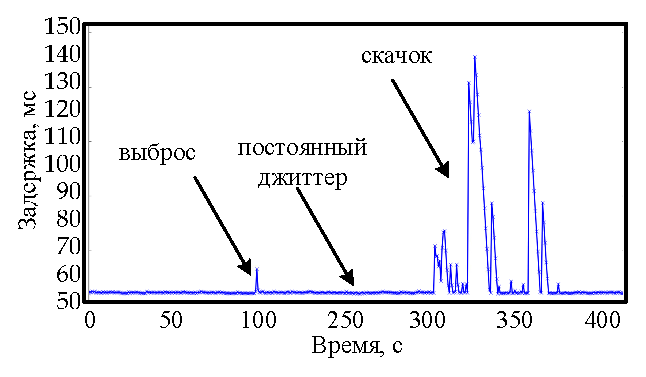
\includegraphics{3typeJitter.eps}
  %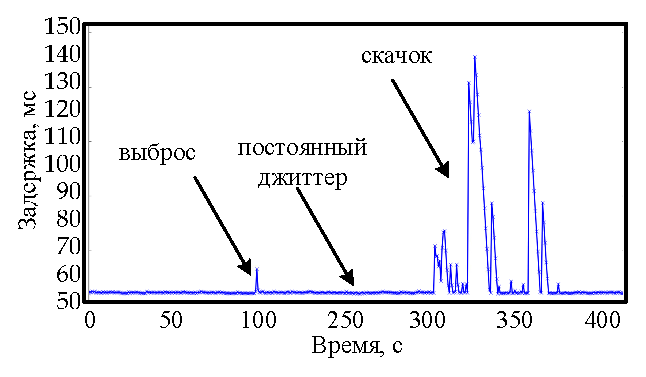
\includegraphics [scale=0.9] {3typeJitter.eps}
%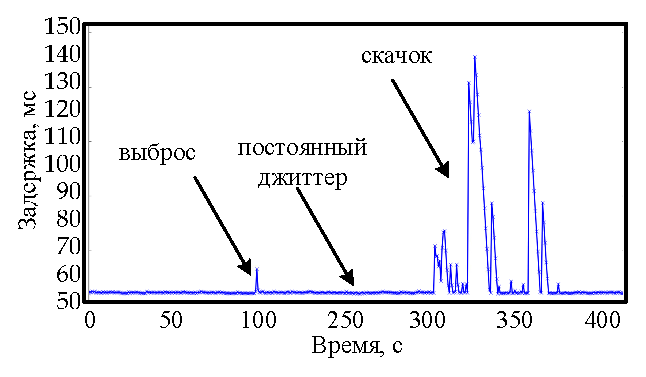
\includegraphics {3typeJitter}
  \caption{Основные типы джиттера пакетной задержки} 
  \label{img:3typeJitter}  
\end{figure}


\section{Анализ причин джиттера в проводной сети} \label{sect2_1}

\subsection{Пакетное планирование на стороне отправителя (тип 1)} \label{subsect2_1_1}
Когда оконечное устройство связи реализовано программно и является частью более общей многофункциональной системы, процессу VoIP приходится бороться за процессорное время с другими процессами и, следовательно, это может привести к некоторому постоянному джиттеру времени передачи.

\subsection{Перегрузка в локальной сети (тип 2)} \label{subsect2_1_2}
Хотя средняя загрузка локальной сети обычно не высокая, локальные перегрузки происходят в течение короткого периода времени. В худшем случае, изменение задержки ограничено максимальным временем повторной попытки использовать сеть Ethernet, а в некоторых системах, также ограничено межпакетным интервалом.
Если VoIP оконечное устройство не было в состоянии получить доступ к локальной сети в течение максимального времени отсрочки или до запланированного момента передачи следующего пакета, то пакет может быть отброшен. В случае 100 Мбит Ethernet максимальное время отсрочки находится в диапазоне миллисекунд и, следовательно, не должны быть основным источником джиттера. В случае 10 Мбит Ethernet максимальное время отсрочки значительно выше, чем временной интервал между голосовыми пакетами и, следовательно, джиттер может быть ограничен временным интервалом между пакетами (обычно около 10-30 мс).
Перегрузки в локальной сети обычно приводят к выбросам задержки так, как если один пакет не получит доступ к сети и будет задержан, следующий пакет сразу может получить доступ к локальной сети (рис. \ref{img:localCongest}).

\begin{figure} [!h]
  \center
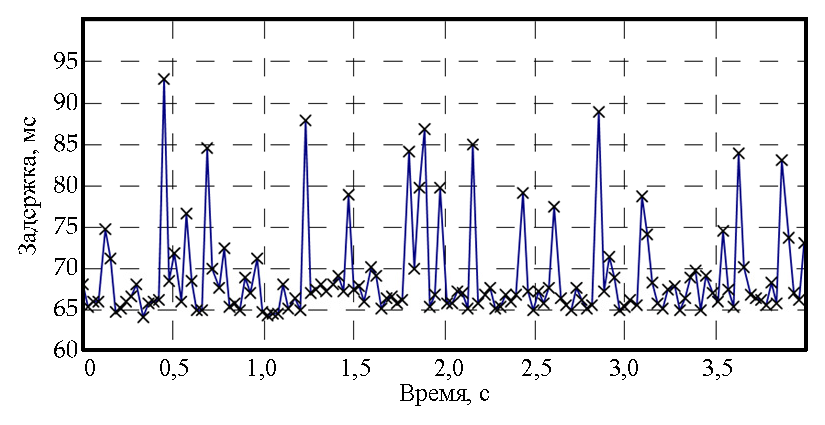
\includegraphics{localCongest.eps}
  \caption{Пример перегрузки в локальной сети \cite{clark}}
  \label{img:localCongest}
\end{figure}

\subsection{Перегрузки в канале доступа (тип 3) } \label{subsect2_1_3}
Доступ к каналу передачи, как правило, является одним из основных источников джиттера, поскольку представляет собой одно из узких мест на пути пакета (рис. \ref{img:accessCongest}). Например, задержка сериализации IP-пакета в 1500 байт, посланного через T1 (1.544Mbit), будет около 8 миллисекунд, поэтому если в очереди перед речевым пакетом находятся пять пакетов данных, то вводится дополнительная задержка в 40 мс. Проблема перегрузок канала доступа может быть еще более серьезной в случае ISDN, ADSL или в случае кабельных модемов, у которых пропускная способность исходящего канала дополнительно ограничена, например, если пропускная способность исходящего канала составляет 384кбит/в секунду, то каждый 1500 байтовый IP пакет в очереди введет дополнительную задержку в 30 мс.

\begin{figure} [!h]
  \center
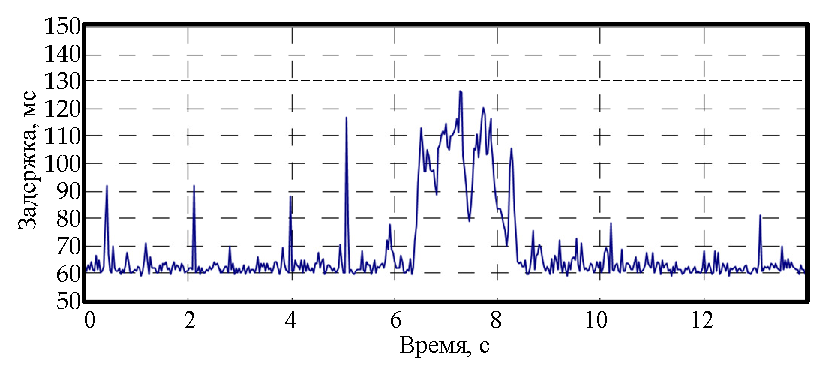
\includegraphics{accessCongest.eps}
  \caption{Пример перегрузки сети доступа \cite{clark}}
  \label{img:accessCongest}
\end{figure}

\subsection{Распределение нагрузки между несколькими линиями доступа или сервис-провайдерами (тип 1) } \label{subsect2_1_4}
В целях предоставления предприятию VoIP доступа, предприятие может быть подключено через несколько сетей доступа к одному сервис-провайдеру или направлять VoIP трафик через несколько независимых провайдеров. Это может привести к джиттеру если задержки на каждом канале доступа существенно различаются.

\subsection{Распределение нагрузки (тип 1) } \label{subsect2_1_5}
Некоторые сервис-провайдеры распределяют трафик через несколько внутренних маршрутов в пределах их сетей в целях повышения устойчивости и обеспечения более равномерной загрузки на сеть. Это вносит джиттер в результате разницы в задержке на каждом маршруте.

\subsection{Внутреннее разделение нагрузки в маршрутизаторах (тип 1) } \label{subsect2_1_6}
Для того чтобы поддерживать высокую скорость обработки некоторые маршрутизаторы используют многопроцессорные подход, при котором пакеты обрабатываются в нескольких параллельных очередях. Это может привести к небольшому уровню джиттера из-за различия в размере очереди.

\subsection{Высокоприоритетный служебный трафик (тип 2) } \label{subsect2_1_7}
Маршрутизаторы периодически генерируют трафик обновления с высоким приоритетом (рис. \ref{img:routeTraffic}) и выполняют обновления таблицы маршрутизации. Каждое такое событие может привести к задержке небольшого количества пакетов. Кроме того во время обновления таблицы маршрутизации могут существовать кратковременные петли, что может привести к чрезвычайно высокой задержке для отдельных пакетов (рис. \ref{img:routeChange}).

\begin{figure} [!h]
  \center
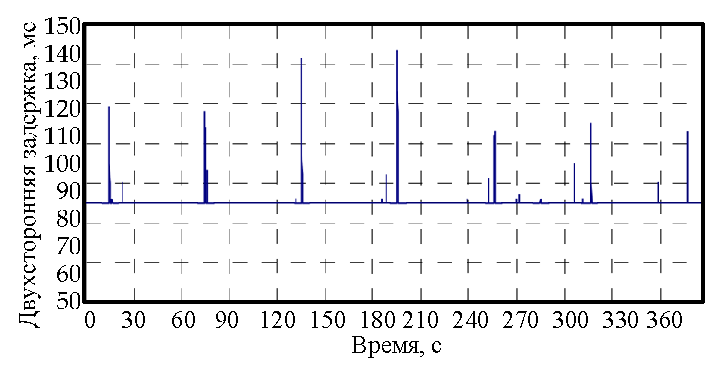
\includegraphics{routeTraffic.eps}
  \caption{Периодическое обновление таблицы маршрутизации без изменения маршрута \cite{clark}}
  \label{img:routeTraffic}
\end{figure}
\begin{figure} [!h]
  \center
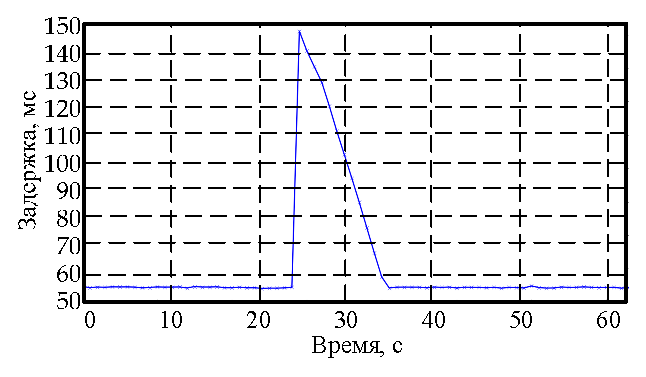
\includegraphics{routeChange.eps}
  \caption{Периодическое обновление таблицы маршрутизации при изменении маршрута \cite{clark}}
  \label{img:routeChange}
\end{figure}

\section{Анализ основных причин джиттера в беспроводной сети LTE} \label{sect2_2}
Беспроводная сеть налагает дополнительные факторы ухудшающие качество передачи. Далее рассмотрим влияние различных факторов на качество обслуживания, для услуг реального времени поверх сети LTE. Для моделирования и анализа ухудшающих факторов воспользуемся сетевым симулятором NS3.

\subsection{Хэндовер}  \label{handover_chapter2}
Хэндовер (англ. Handover), является процессом передачи сессии абонента от одной базовой станции к другой. Может быть, несколько причин для проведения передачи сессии:
\begin{itemize}
\item Когда абонент уходит с зоны покрытия одной ячейкой сети и входит в зону покрытия другой ячейкой. Хэндовер позволяет абонентам не быть привязанным к какой-либо географической точке и дает возможность передвигаться в пределах сети оператора без разрыва соединения.
\item Когда ёмкость сети в текущей ячейке израсходована при существовании соединения, которое находится в зоне, перекрытой другой ячейкой, передаётся к этой ячейке в порядке освобождения ёмкости первой ячейки для других ее пользователей, которые могут быть соединены только с первой ячейкой.
\item Когда канал используемый абонентом сильно зашумлён помехами, соединение передаётся другому каналу в той же ячейке или другому каналу в другой ячейке для устранения помех.
\item Когда абонент входит в зону микроячейки, соединение может быть передано для освобождения емкости большой сети.
\end{itemize}
Проведем моделирование влияния хэндовера на сквозную задержку в сети LTE в сетевом симуляторе NS3.
На рис. \ref{img:hand} изображено изменение сквозной сетевой задержки прибытия пакетов из-за 3-х переключений сессии абонента между базовыми станциями, выполненными через некоторый промежуток времени.
Также стоит заметить, что при первой установке соединения задержка прибытия пакетов тоже была не стационарна.
\nomenclature{NS3}{Network Simulator 3}
\begin{figure} [h]
  \center
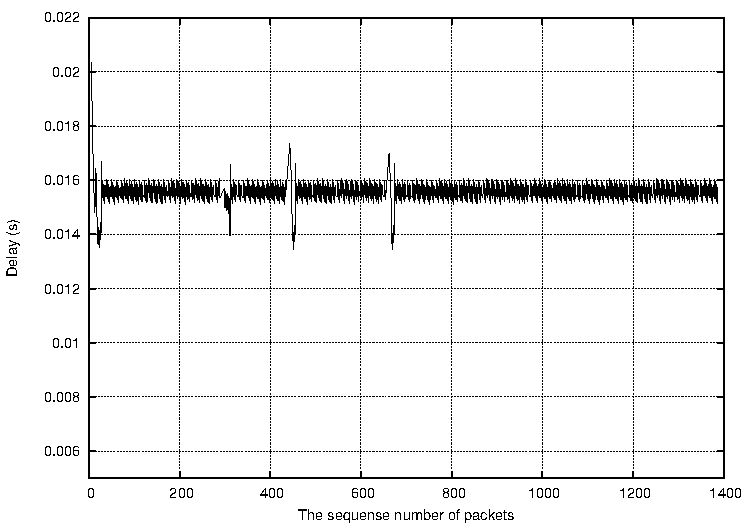
\includegraphics{hand-eps-converted-to.pdf}
  \caption{Изменение задержки прибытия пакетов при хэндовере между базовыми станциями}
  \label{img:hand}
\end{figure}

\subsection{Расстояния между абонентом и базовой станцией}  \label{sect2_2_2}
Проведем моделирование влияния расстояния между абонентом и базовой станцией на скорость передачи в канале сети LTE в сетевом симуляторе NS3.



Уравнение передачи для радиолинии протяженностью $d$ \cite{Friis}:
\begin{equation}\label{eq:friisNew}
P_{r}=\frac{P_{t}G_{t}G_{r}\lambda^{2}}{(4\pi d)^{2}L},
\end{equation}

\noindent где $P_{r}$ - мощность полученного сигнала (Вт), $P_{t}$ - мощность отправленного сигнала (Вт), $G_{t}$ - коэффициент передачи, $G_{r}$ - коэффициент приема, $\lambda$ - длина волны (м), $d$ - расстояние (м), $L$ - системные потери. Очевидно (рис. \ref{img:dist} (a)) с увеличением расстояния между абонентом и базовой станцией уменьшается отношение сигнал шум с внутрисистемными помехами включительно (SINR). Вместе с тем, с уменьшением SINR также уменьшается и MCS и TBS (рис. \ref{img:dist} (b,c))

Для расчета пропускной способности канала воспользуемся спектральной эффективностью $\eta_{i}$ из табл. \ref{MCS_spectr}  \cite{R1-081483}. Которая рассчитывается по формуле:

\begin{equation}\label{eq:spectr1}
\eta_{i}=log_{2}(1+\frac{\gamma_{i}}{\Gamma}),
\end{equation}
\begin{equation}\label{eq:spectr2}
\Gamma=\frac{-ln(5\times BER}{1.5},
\end{equation}
\begin{equation}\label{eq:spectr3}
BER=0.00005.
\end{equation}

Рассчитанная пропускная способность канала при ширине спектра канала  20МГц изображена на рис. \ref{img:dist} (d).

\clearpage


\begin{longtable}{|l|l|l|l|}
\caption{Соотношение спектральной эффективности ($\eta_{i}$) к индексу MCS ($I_{MCS}$)}\label{MCS_spectr}
 \hline
 \hline
Спектральная эффективность($\eta_{i}$) & $Q_{m}$ & $R$        & MCS индекс ($I_{MCS}$) \\ \hline 



    \endfirsthead   \hline
 \multicolumn{4}{c|}{\small\slshape (продолжение)}        \\ \hline
Спектральная эффективность($\eta_{i}$) & $Q_{m}$ & $R$        & MCS индекс ($I_{MCS}$)   \\ \hline
        
                                              \endhead        \hline
 \multicolumn{4}{r|}{\small\slshape продолжение следует}  \\ \hline
                                              \endfoot        \hline
                                              \endlastfoot





\multicolumn{3}{|l|}{Reserved}  & 0 \\  \hline
    0.15234375     & 2  & 0.076172 & 1       \\ \hline
    0.193359375    & 2  & 0.09668  & 2       \\ \hline
    0.234375       & 2  & 0.117188 & 3       \\ \hline
    0.305664063    & 2  & 0.152832 & 4       \\ \hline
    0.376953125    & 2  & 0.188477 & 5       \\ \hline
    0.489257813    & 2  & 0.244629 & 6       \\ \hline
    0.6015625      & 2  & 0.300781 & 7       \\ \hline
    0.739257813    & 2  & 0.369629 & 8       \\ \hline
    0.876953125    & 2  & 0.438477 & 9       \\ \hline
    1.026367188    & 2  & 0.513184 & 10      \\ \hline
    1.17578125     & 2  & 0.587891 & 11      \\ \hline
    1.326171875    & 4  & 0.331543 & 12      \\ \hline
    1.4765625      & 4  & 0.369141 & 13      \\ \hline
    1.6953125      & 4  & 0.423828 & 14      \\ \hline
    1.9140625      & 4  & 0.478516 & 15      \\ \hline
    2.16015625     & 4  & 0.540039 & 16      \\ \hline
    2.40625        & 4  & 0.601563 & 17      \\ \hline
    2.568359375    & 4  & 0.64209  & 18      \\ \hline
    2.73046875     & 6  & 0.455078 & 19      \\ \hline
    3.026367188    & 6  & 0.504395 & 20      \\ \hline
    3.322265625    & 6  & 0.553711 & 21      \\ \hline
    3.612304688    & 6  & 0.602051 & 22      \\ \hline
    3.90234375     & 6  & 0.650391 & 23      \\ \hline
    4.212890625    & 6  & 0.702148 & 24      \\ \hline
    4.5234375      & 6  & 0.753906 & 25      \\ \hline
    4.819335938    & 6  & 0.803223 & 26      \\ \hline
    5.115234375    & 6  & 0.852539 & 27      \\ \hline
    5.334960938    & 6  & 0.88916  & 28      \\ \hline
    5.5546875      & 6  & 0.925781 & 29      \\ \hline
    2.4            & 2  & 1.2      & 30      \\ \hline
\multicolumn{3}{|l|}{Reserved}  & 31 \\  \hline
    \end{longtable}




\begin{figure} [!h]
\begin{minipage}[h]{0.47\linewidth}
\center
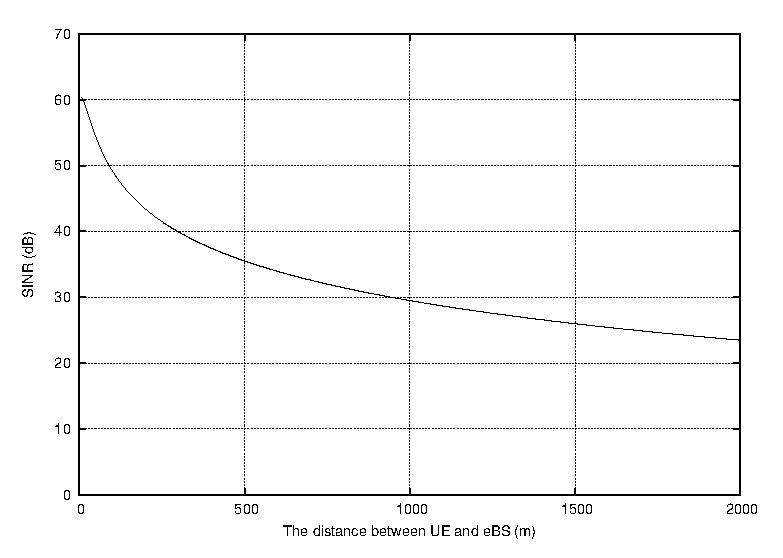
\includegraphics[width=1\linewidth]{Sinr_dist.eps} a) \\
\end{minipage}
\hfill
\begin{minipage}[h]{0.47\linewidth}
\center
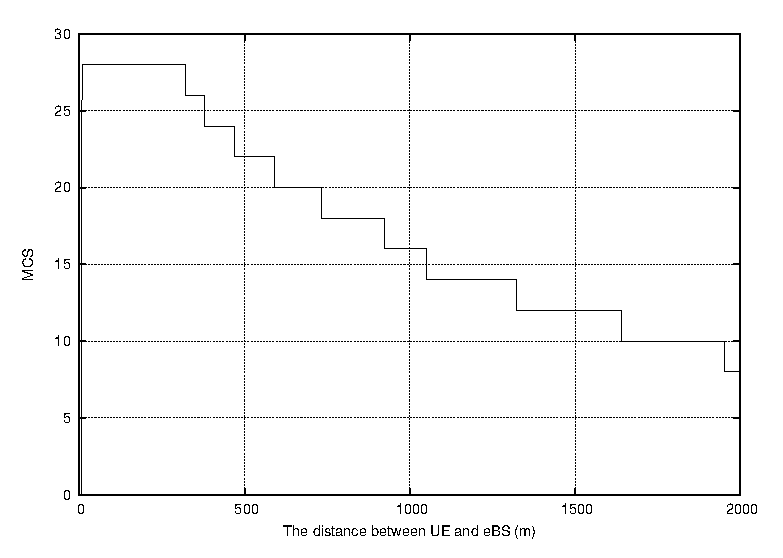
\includegraphics[width=1\linewidth]{mcs_dist.eps} b) \\
\end{minipage}
\vfill
\begin{minipage}[h]{0.47\linewidth}
\center
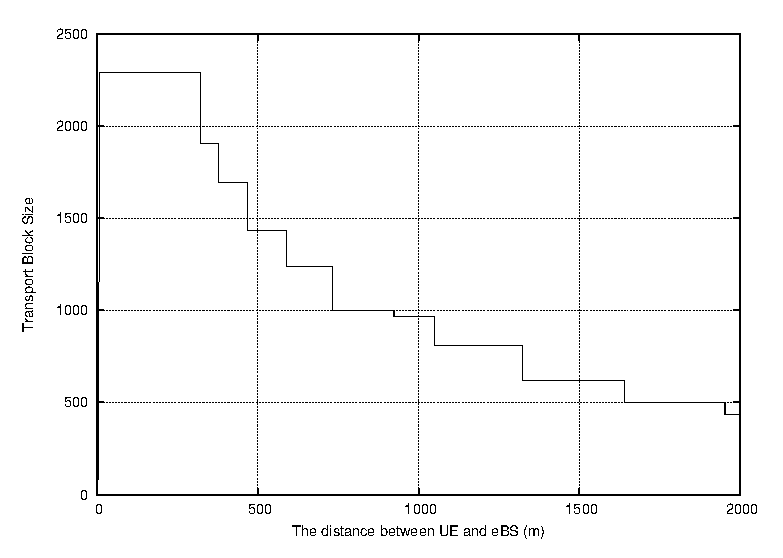
\includegraphics[width=1\linewidth]{tb_dist.eps} c) \\
\end{minipage}
\hfill
\begin{minipage}[h]{0.47\linewidth}
\center
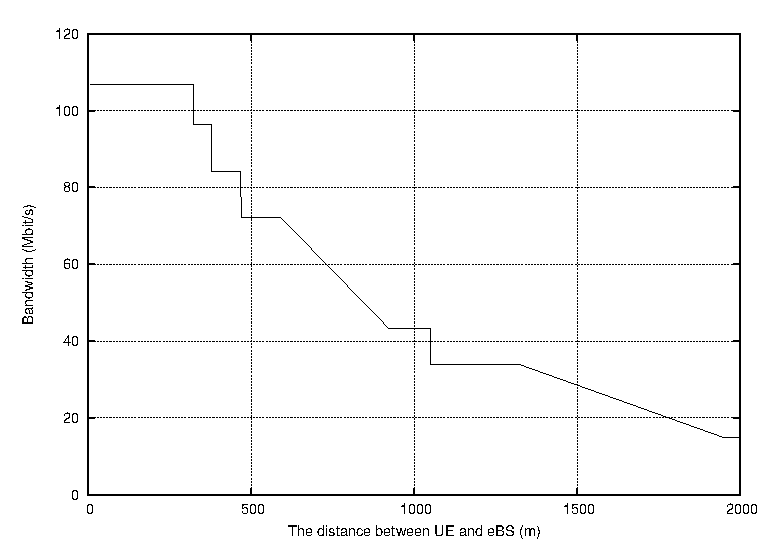
\includegraphics[width=1\linewidth]{speed_dist.eps} d) \\
\end{minipage}
\caption{Зависимость a) SINR b) MCS c) размера TBS d) скорости передачи нисходящего канала передачи от расстояния между абонентом и базовой станцией}
\label{img:dist}
\end{figure}

\subsection{Внутрисистемные помехи}  \label{sect2_2_3}
Рассмотрим влияние всплесков внутрисистемных помех на характеристики канала передачи в сети LTE. Наличие этих помех определяет суть проблемы электромагнитной совместимости. 
Выброс внутрисистемных помех может быть вызван влиянием соседней базовой станции, которая работает в том же диапазоне.
Анализ показывает, что выбросы помех влияют на характеристики канала, в том числе на джиттер и потери пакетов.
\nomenclature{FTP}{File Transfer Protocol}
Для борьбы с внутрисистемными помехами используются различные методы: уход на другую частоту, помехоустойчивое кодирование и перемежение. 
Тем не менее, с ухудшением условий расспространения волны возникают блоковые ошибки. 
Это приводит к потере пакетов для IP услуг, таких как FTP и VoIP. В технологии LTE приходится использовать повторные передачи, чтобы потери пакетов не снижались ниже определенного уровня, однако эта мера может быть не достаточно эффективной, чтобы предоставить хорошее качество для соответствующей услуги. В результате использования повторных передач появляется джиттер задержки.
LTE передачи обычно планируются таким образом, чтобы быть синхронизированными с качеством канала. При этом пакеты передаются к и от пользователей, имеющих наилучшие канальные условия, а пользователи, которые испытывают провалы качества канала, будут ожидать пока условия канала не будут улучшены. Это означает, что пакеты в очереди передачи будут испытывать различные задержки из-за планирования.
LTE также ограничивает количество повторных передач, чтобы избежать расхода слишком большого количества ресурсов передачи для тех пользователей, которые испытывают деградацию условий канала. Это означает, что потери пакетов могут происходить в дополнение к джиттеру задержки. Для услуг реального времени, характерно чтобы пакеты могли быть повторно переданы со сквозной задержкой до 50-100 мс.
Пример задержек пакетов, которые могут произойти в присутствии внутрисистемных помех, показан на рис \ref{img:example_inter}.


\pgfplotsset{width=15cm, height=10cm, compat=1.3}
\begin{figure} [h]
  \center
\begin{tikzpicture}
\begin{axis}[
xlabel=Номер пакета,
ylabel=Задержка пакета (мс)]
\addplot [only marks, color=blue ,mark=x] coordinates {
( 1, 150 )
( 2, 150 )
( 3, 150 )
( 4, 150 )
( 5, 150 )
( 6, 150 )
( 7, 150 )
( 8, 150 )
( 9, 150 )
( 13, 250 )
( 14, 230 )
( 15, 210 )
( 16, 190 )
( 17, 170 )
( 19, 150 )
( 20, 150 )
( 21, 150 )
( 22, 150 )
( 21, 150 )
( 22, 150 )
( 23, 150 )
( 24, 150 )
( 25, 150 )
( 26, 150 )
( 27, 150 )
( 28, 150 )
( 29, 150 )
( 30, 150 )


};
\addplot [only marks, color=red] coordinates {
( 10, 0 )
( 11, 0 )
( 12, 0 )};
\legend{Задержка пакета, Потеря пакета}
\end{axis}
\end{tikzpicture}
\caption{Пример времени прибытия IP пакетов (крестообразные маркеры), потерь пакетов (круглые маркеры) и джиттера задержки в присутствии сильного всплеска внутрисистемных помех.}
  \label{img:example_inter}
\end{figure}



До воздействия внутрисистемной помехи пакеты передаются без или почти без джиттера. В этом примере предполагается, что постоянный джиттер отсутствует, чтобы выделить влияние помехи на задержку прибытия пакетов.
На начальном этапе воздействия помехи пакеты обычно теряются. Это происходит из-за ограничений в планировании передачи пакетов и ограничений времени повторной передачи, как описано выше.
Пакеты, сгенерированные в конце периода воздействия помехи, будут поставлены в очередь. Вероятней всего, отправка пакетов будет успешной только после окончания периода влияния помехи. 
Это может привести к большим задержкам этих пакетов. 
Вероятным следствием длительных задержек пакетов является то, что буфер компенсации джиттера отбросит пакеты, которые пришли слишком поздно.
После периода воздействия помехи задержки пакетов медленно снижаются. Это потому, что пакеты, которые сгенерированные непосредственно после помехи еще ожидают в очереди передачи.
Передача вернется к нормальному состоянию, когда передатчик очистит очередь передачи.
Скачок задержки после влияния помехи является довольно частым явлением в пакетнокоммутируемой сотовой сети, которая использует повторные передачи. 
Величина потерь пакетов и размер скачка задержки зависит как от помехи так и от того как система настроена.

Проведем моделирование влияния внутрисистемных помех на параметры передачи пакетов в сети LTE. Схема моделирования в NS3 изображена на рис. \ref{img:inter_schem}. С уменьшением расстояния до источника помехи, мощность помехи увеличивается, и характеристики канала начинают деградировать, когда SINR достигает некоего критического уровня (рис. \ref{img:inter}).
Из рис. \ref{img2:inter_del}-\ref{img2:inter_drop} видно, что чем больше скорость передачи потока, тем значительнее увеличивается джиттер и пакетные потери из-за влияния внутрисистемной помехи.
\begin{figure} [!h]
  \center
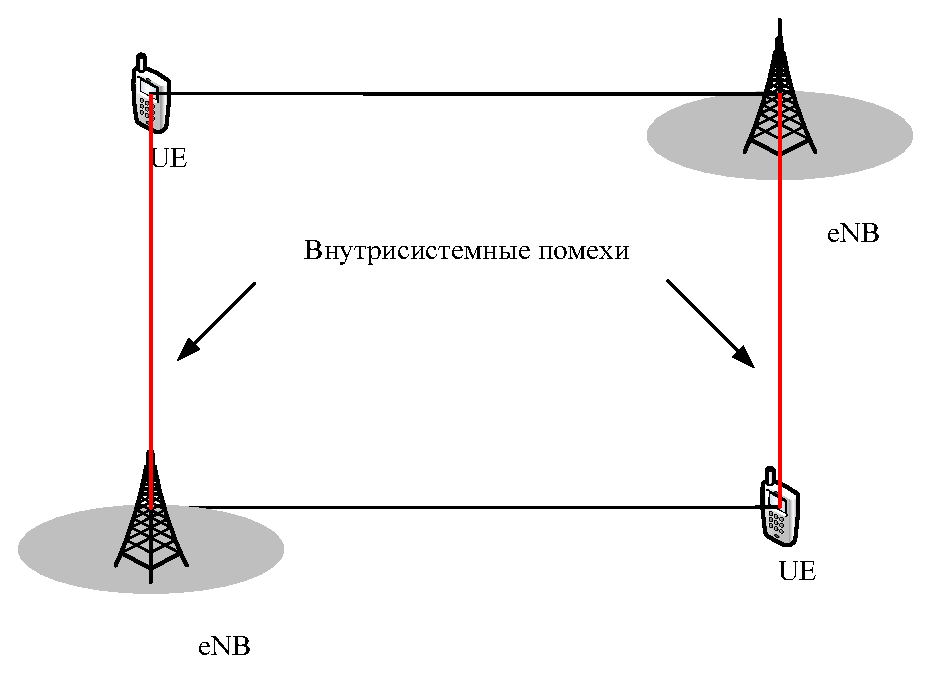
\includegraphics[width=0.6\linewidth]{inter_schem.eps}
  \caption{Схема моделирования влияния внутрисистемных помех в NS3}
  \label{img:inter_schem}
\end{figure}
\begin{figure} [!h]
\begin{minipage}[h]{0.47\linewidth}
\center
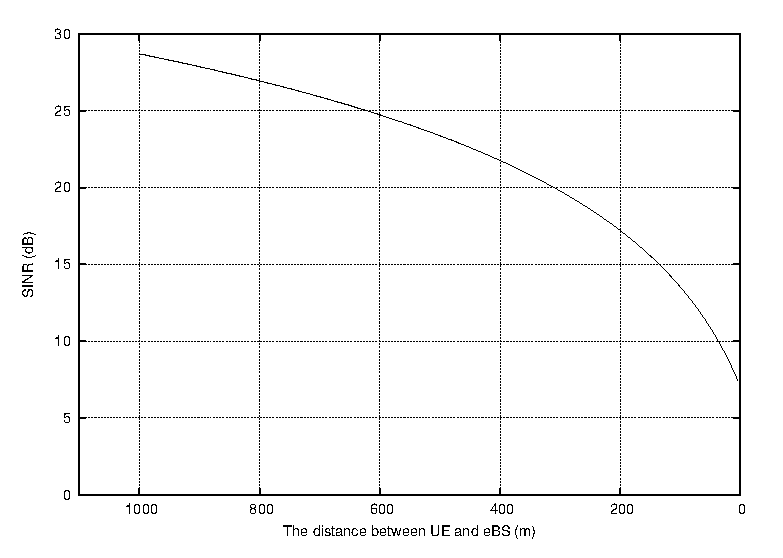
\includegraphics[width=1\linewidth]{Sinr_inter.eps} a) \\
\end{minipage}
\hfill
\begin{minipage}[h]{0.47\linewidth}
\center
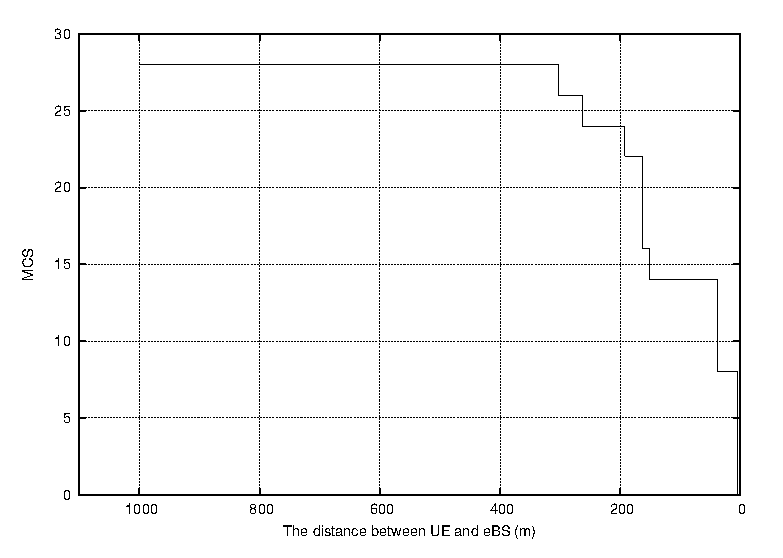
\includegraphics[width=1\linewidth]{mcs_inter.eps} b) \\
\end{minipage}
\vfill
\begin{minipage}[h]{0.47\linewidth}
\center
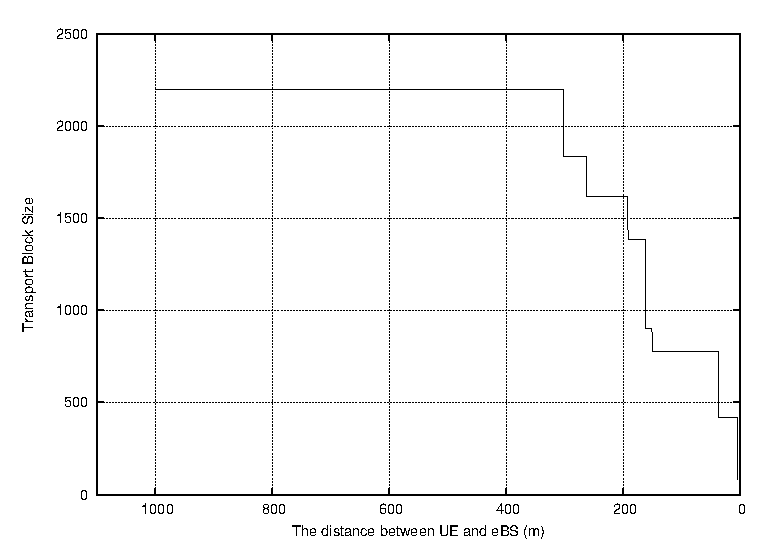
\includegraphics[width=1\linewidth]{tb_inter.eps} c) \\
\end{minipage}
\hfill
\begin{minipage}[h]{0.47\linewidth}
\center
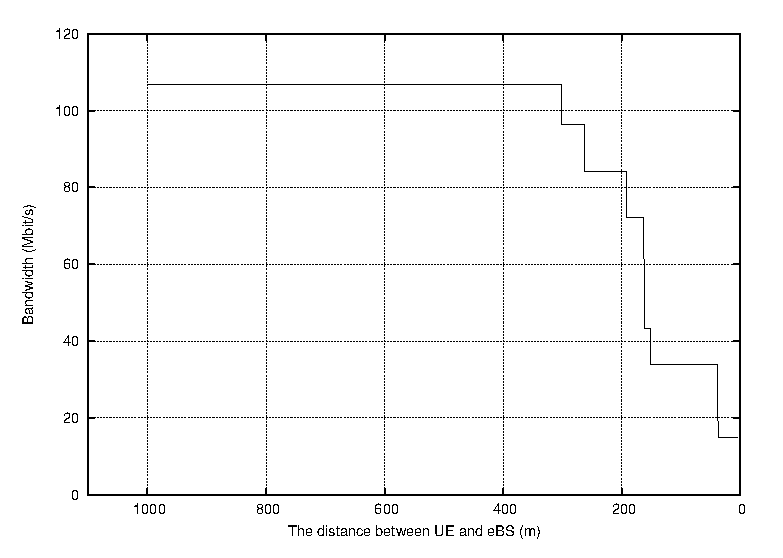
\includegraphics[width=1\linewidth]{speed_inter.eps} d) \\
\end{minipage}
\caption{Зависимость a) SINR b) MCS c) размера TB d) скорости передачи нисходящего канала передачи от расстояния между абонентом и помеховой базовой станцией}
\label{img:inter}
\end{figure}
\nomenclature{SINR}{Signal to Interference plus Noise Ratio}
\nomenclature{MCS}{Modulation and Coding Scheme}
\nomenclature{TB}{Transport Block}


\pgfplotsset{width=15cm, height=10cm, compat=1.3}
\begin{figure} [!h]
  \center
\begin{tikzpicture}
%\pgfkeys{/pgfplots/legend pos=north west}

\begin{axis}[
mark options={scale=0.7},
ylabel={Mem [GB]},
legend style={
%area legend,
at={(0.5,-0.2)},
anchor=north,
legend columns=3},
legend cell align=left,
cycle list name=mark list,
%cycle list name=linestyles,
xlabel=Расстояние до источника внутрисистемной помехи (м),
ylabel=Джиттер (мс),
x dir=reverse
]

\addplot coordinates {
(1000,0)
(500,0)
(300,0)
(100,0.1)
(50,0.16)};
\addplot coordinates {
(1000,0.34)
(500,0.36)
(300,0.38)
(100,0.7)
(50,0.74)};
\addplot coordinates {
(1000,0.4)
(500,0.4)
(300,0.4)
(100,0.71)
(50,0.75)};


\legend{512кБ/с, 2МБ/с, 3МБ/с}
\end{axis}
\end{tikzpicture}
\caption{Зависимость джиттера от расстояния до источника внутрисистемной помехи}
  \label{img2:inter_del}
\end{figure}


\pgfplotsset{width=15cm, height=10cm, compat=1.3}
\begin{figure} [!h]
  \center
\begin{tikzpicture}
%\pgfkeys{/pgfplots/legend pos=north west}

\begin{axis}[
mark options={scale=0.7},
ylabel={Mem [GB]},
legend style={
%area legend,
at={(0.5,-0.2)},
anchor=north,
legend columns=3},
legend cell align=left,
cycle list name=mark list,
%cycle list name=linestyles,
xlabel=Расстояние до источника внутрисистемной помехи (м),
ylabel=Пакетные потери (\%),
x dir=reverse
]

\addplot coordinates {
(1000,0)
(500,0)
(300,0)
(100,2.8)
(50,3.1)};
\addplot coordinates {
(1000,2.8)
(500,2.8)
(300,2.8)
(100,5.3)
(50,6.5)};
\addplot coordinates {
(1000,3.1)
(500,3.1)
(300,3.1)
(100,5.8)
(50,7.0)};
\legend{512кБ/с, 2МБ/с, 3МБ/с}
\end{axis}
\end{tikzpicture}
\caption{Зависимость пакетных потерь от расстояния до источника внутрисистемной помехи}
  \label{img2:inter_drop}
\end{figure}



\subsection{Замирания в канале}  \label{sect2_2_4}
\nomenclature{MIMO}{Multiple-Input and Multiple-Output}
Работа LTE-приемника зависит от разных факторов: конкретного частотного диапазона, многолучевых задержек, доплеровских сдвигов частоты, реализации технологии множественного приема/передачи (MIMO) и т.д.

В реальной среде такие объекты, как горы, здания и машины, отражают, преломляют или не пропускают передаваемые радиосигналы. Эти объекты могут располагаться на различном расстоянии от передатчика – одни ближе, другие дальше. Вследствие этого множество копий сигнала достигают антенны приемника за разное время. У таких запаздывающих копий разные фазовые соотношения, которые при приеме дают как положительный, так и отрицательный эффект. Незначительные отклонения в фазовых соотношениях вызывают пешеходы и машины. Если абонентский терминал перемещается, то изменение фазы увеличивается с ростом его скорости.

Эксперименты показывают колебания уровня принимаемого сигнала выше или ниже его номинала; иногда он снижается до очень низких, почти нулевых значений.

При движении передатчика или приемника проявляется другой эффект – доплеровский сдвиг частоты. Так как запаздывающие копии сигнала поступают на приемник с разных относительно вектора движения направлений, частоты некоторых из них сдвигаются – одни выше, другие ниже реальной частоты сигнала. Этот эффект вызывает особые сложности в OFDM-системах, поскольку для устранения интерференции внутренних поднесущих нельзя использовать простой сдвиг частоты.

По мере увеличения количества путей распространения сигнала растет и число наложений его копий с разной синхронизацией, амплитудой, частотой и фазой. В результате сигнал становится стохастическим (недетерминированным) с рэлеевским распределением. Как известно, рэлеевское распределение достаточно точно отображает колебания амплитуды и изменения частоты (называемые еще доплеровским расширением), характерные для городской застройки.

Условия распространения характеризуются тремя факторами: профилем многолучевой задержки, доплеровским расширением и, в случае применения нескольких антенн, – набором коррелирующих матриц, задающих соотношения для передающей и приемной антенн.

Профиль задержки определяет количество путей распространения, саму задержку и ослабление сигнала. Кроме того, по этому профилю можно вычислить среднеквадратичное отклонение (разброс) задержки. Для технологии LTE выбраны три профиля: для пешехода (табл. \ref{EPA}), мобильного пользователя в автомобиле (табл. \ref{EVA}) и для типовой городской застройки (табл. \ref{ETU}). Суммарная информация по профилям задержек для технологии LTE находится в табл. \ref{ProfileDelay}.

\nomenclature{eNB}{E-UTRAN Node B}
\nomenclature{OFDM}{Orthogonal Frequency-Division Multiplexing}

\nomenclature{EPA}{Extended Pedestrian A Model}
\nomenclature{EVA}{Extended Vehicular A Model}
\nomenclature{ETU}{Extended Typical Urban model}

\begin{table} [htb]
  \centering
\parbox{15cm}{\caption{Расширенная А модель пешехода (ЕРА) \cite{TS36104}}\label{EPA}}
\begin{tabular}{|p{7cm}|p{7cm}|}
    \hline
    \hline
    Задержка за счет отклонения от трассы в нс &  Соответствующая мощность в дБ \\ \hline \hline
    0                                     & 0.0                           \\ \hline
    30                                    & -1.0                          \\ \hline
    70                                    & -2.0                          \\ \hline
    90                                    & -3.0                          \\ \hline
    110                                   & -8.0                          \\ \hline
    190                                   & -17.2                         \\ \hline
    410                                   & -20.8                         \\ \hline
    \end{tabular}

\end{table}

\begin{table} [htb]
  \centering
\parbox{15cm}{\caption{Расширенная А-модель при движении в автомобиле (EVA) \cite{TS36104}}\label{EVA}}
\begin{tabular}{|p{7cm}|p{7cm}|}
    \hline
    \hline
    Задержка за счет отклонения от трассы в нс &  Соответствующая мощность в дБ \\ \hline \hline
    0                                          & 0.0                           \\ \hline
    30                                         & -1.5                          \\ \hline
    150                                        & -1.4                          \\ \hline
    310                                        & -3.6                          \\ \hline
    370                                        & -0.6                          \\ \hline
    710                                        & -9.1                          \\ \hline
    1090                                       & -7.0                          \\ \hline
    1730                                       & -12.0                         \\ \hline
    2510                                       & -16.9                         \\ \hline
    \end{tabular}
\end{table}


\begin{table} [htb]
  \centering
\parbox{15cm}{\caption{Расширенная модель для типовой городской застройки (ETU) \cite{TS36104}}\label{ETU}}
\begin{tabular}{|p{7cm}|p{7cm}|}
    \hline
    \hline
    Задержка за счет отклонения от трассы в нс &  Соответствующая мощность в дБ \\ \hline \hline
    0    & -1.0 \\ \hline
    50   & -1.0 \\ \hline
    120  & -1.0 \\ \hline
    200  & 0.0  \\ \hline
    230  & 0.0  \\ \hline
    500  & 0.0  \\ \hline
    1600 & -3.0 \\ \hline
    2300 & -5.0 \\ \hline
    5000 & -7.0 \\ \hline
    \end{tabular}
\end{table}



\begin{table} [htb]
  \centering
\parbox{15cm}{\caption{Профили задержек для технологии LTE \cite{iks}}\label{ProfileDelay}}
    \begin{tabular}{|p{4cm}|p{3cm}|p{3cm}|p{4cm}|}
    \hline \hline
    Модель                                                            &  Количество путей в канале &  Разброс задержки в нс &  Максимальная задержка по траектории в нс \\ \hline \hline
    Расширенная А-модель пешехода (ЕРА)                               & 7                          & 45                     & 410                                       \\ \hline
    Расширенная А-модель при движении в автомобиле (EVA) & 9                          & 367                    & 2510                                      \\ \hline
    Расширенная модель для типовой городской застройки (ETU)          & 9                          & 991                    & 5000                                      \\ \hline
    \end{tabular}
\end{table}



Еще один параметр – максимальная величина доплеровского сдвига частоты. Он имеет частотный сдвиг:

\begin{equation}\label{eq:maxDeltaF}
f_{D}=\frac{\mathcal{V}}{c}-f_{c},
\end{equation}
\noindent где $f_{c}$ является несущей частотой, $\mathcal{V}$ - скорость движения антены и $c$ - скорость света. Все пути в канале имеют классический доплеровский спектр плотности мощности:

\begin{equation}\label{eq:maxDeltaF1}
S(f)=\frac{1}{\pi f_D \sqrt{1-(\frac{f}{f_D})^2}},
\end{equation}
\noindent где $f\epsilon [-f_D;f_D]$. Для LTE-сетей обычно применяются три значения: 5 Гц, 70 Гц и 300 Гц – для низко, средне и высокоскоростных объектов. При работе в диапазоне 2 ГГц эти частоты соответствуют следующим скоростям движения пользовательского терминала: 2,7 км/ч, 38,4 км/ч и 162 км/ч. Требования к работе приемника формируются с учетом комбинации этих доплеровских сдвигов частоты с профилями задержки. И хотя существуют три профиля и три доплеровских сдвига частоты, из возможных сочетаний используются пять (табл. \ref{model_chanel}). Профиль пешехода как низкоскоростного объекта определен только для частоты 5 Гц; профиль пользователя в автомобиле – для 5 и 70 Гц, а типовой профиль для города не включает частоту 5 Гц.






Проведем моделирование влияния замираний сигнала в LTE. Влияние замираний на характеристики нисходящего канала передачи при пешеходном сценарии (0-3 км/ч) изображено на рис. \ref{img:EPA_3kmph}. Влияние замираний на характеристики нисходящего канала передачи при автомобильном сценарии (30-60 км/ч) изображено на рис. \ref{img:EVA_60kmph}.

Замирания в канале, в конечном счете, влияют на прикладной уровень услуг. Далее представим результаты моделирующего эксперимента, проведенного в сетевом симуляторе NS3, который демонстрирует влияние различных типов замирания на задержку, джиттер и пакетные потери в зависимости от расстояния между абонентом и базовой станцией (рис. \ref{img2:fad_del}-\ref{img2:fad_drop}).

\begin{figure} [!h]
\begin{minipage}[h]{0.47\linewidth}
\center
\includegraphics[width=1\linewidth]{EPA_3kmph/Sinr_fading.eps} a) \\
\end{minipage}
\hfill
\begin{minipage}[h]{0.47\linewidth}
\center
\includegraphics[width=1\linewidth]{EPA_3kmph/mcs_fading.eps} b) \\
\end{minipage}
\vfill
\begin{minipage}[h]{0.47\linewidth}
\center
\includegraphics[width=1\linewidth]{EPA_3kmph/tb_fading.eps} c) \\
\end{minipage}
\hfill
\begin{minipage}[h]{0.47\linewidth}
\center
\includegraphics[width=1\linewidth]{EPA_3kmph/speed_fading.eps} d) \\
\end{minipage}
\caption{Влияние замираний на a) SINR b) MCS c) размер TB d) скорость передачи нисходящего канала передачи при пешеходном сценарии (EPA 0-3 км/ч)}
\label{img:EPA_3kmph}
\end{figure}


\begin{table} [!htb]
  \centering
\parbox{15cm}{\caption{Параметры модели канала \cite{iks}}\label{model_chanel}}
\begin{tabular}{|l|c|}
    \hline
    \hline
    Модель     & Максимальный доплеровский сдвиг частоты, Гц \\ \hline \hline
    ЕРА 5 Гц   & 5                                       \\ \hline
    EVA 5 Гц   & 5                                       \\ \hline
    EVA 70 Гц  & 70                                      \\ \hline
    ETU 70 Гц  & 70                                      \\ \hline
    ETU 300 Гц & 300                                     \\ \hline
    \end{tabular}
\end{table}

На рис. \ref{img2:fad_dj} изображено изменение джиттера в зависимости от расстояния для трех профилей задержки: EPA, EVA, ETU. 
При моделировании между абонентом и базовой станцией передается поток со скоростью 512кБ/с. Как мы видим в нашем случае, джиттер и пакетные потери, существенно увеличиваются с увеличением расстояния и при замираниях в канале, которые соответствуют профилю EVA и ETU, даже на небольшом расстоянии предоставление каких либо услуг становится невозможным.

\begin{figure} [!h]
\begin{minipage}[h]{0.47\linewidth}
\center
\includegraphics[width=1\linewidth]{EVA_60kmph/Sinr_fading.eps} a) \\
\end{minipage}
\hfill
\begin{minipage}[h]{0.47\linewidth}
\center
\includegraphics[width=1\linewidth]{EVA_60kmph/mcs_fading.eps} b) \\
\end{minipage}
\vfill
\begin{minipage}[h]{0.47\linewidth}
\center
\includegraphics[width=1\linewidth]{EVA_60kmph/tb_fading.eps} c) \\
\end{minipage}
\hfill
\begin{minipage}[h]{0.47\linewidth}
\center
\includegraphics[width=1\linewidth]{EVA_60kmph/speed_fading.eps} d) \\
\end{minipage}
\caption{Влияние замираний на a) SINR b) MCS c) размер TB d) скорость передачи нисходящего канала передачи при автомобильном сценарии (EVA 30-60 км/ч)}
\label{img:EVA_60kmph}
\end{figure}


\pgfplotsset{width=15cm, height=7cm, compat=1.3}
\begin{figure} [!h]
  \center
\begin{tikzpicture}
\pgfkeys{/pgfplots/legend pos=north west}
\begin{axis}[
mark options={scale=0.7},
legend cell align=left,
%cycle list name=mark list,
cycle list name=linestyles*,
xlabel=Расстояние между абонентом и базовой станцией (м),
ylabel=Задержка (с),
]
\addplot coordinates {
(500,0.04)
(0,0.022)};
\addplot coordinates {
(500,0.053)
(0,0.022)};
\addplot coordinates {
(500,0.035)
(0,0.022)};
\legend{EVA, ETU, EPA}
\end{axis}
\end{tikzpicture}
\caption{Зависимость задержки пакетов от расстояния между абонентом и базовой станцией при замираниях}
  \label{img2:fad_del}
\end{figure}



\pgfplotsset{width=15cm, height=7cm, compat=1.3}
\begin{figure} [!h]
  \center
\begin{tikzpicture}
\pgfkeys{/pgfplots/legend pos=north west}
\begin{axis}[
mark options={scale=0.7},
legend cell align=left,
%cycle list name=mark list,
cycle list name=linestyles*,
xlabel=Расстояние между абонентом и базовой станцией (м),
ylabel=Джиттер (мс),
]
\addplot coordinates {
(500,50)
(0,0.33)};
\addplot coordinates {
(500,57)
(0,0.53)};
\addplot coordinates {
(500,20)
(0,0.31)};
\legend{EVA, ETU, EPA}
\end{axis}
\end{tikzpicture}
\caption{Зависимость джиттера от расстояния между абонентом и базовой станцией при замираниях}
  \label{img2:fad_dj}
\end{figure}


\pgfplotsset{width=15cm, height=7cm, compat=1.3}
\begin{figure} [!h]
  \center
\begin{tikzpicture}
\pgfkeys{/pgfplots/legend pos=north west}
\begin{axis}[
mark options={scale=0.7},
legend cell align=left,
%cycle list name=mark list,
cycle list name=linestyles*,
xlabel=Расстояние между абонентом и базовой станцией (м),
ylabel=Пакетные потери (\%),
]
\addplot coordinates {
(500,53)
(0,2.7)};
\addplot coordinates {
(500,60)
(0,3.7)};
\addplot coordinates {
(500,23)
(0,0.9)};
\legend{EVA, ETU, EPA}
\end{axis}
\end{tikzpicture}
\caption{Зависимость пакетных потерь от расстояния между абонентом и базовой станцией при замираниях}
  \label{img2:fad_drop}
\end{figure}


\section{Синтез математической модели процесса задержки} \label{sect3_1}
Перед синтезом алгоритма буфера компенсации джиттера необходимо определится с моделью задержки, которая представляет собой случайный гауссовский процесс. 
Достаточно конструктивной моделью случайного динамического процесса, является процесс $x(t)$ на выходе формирующего фильтра, описываемого уравнением состояния:

\begin{equation}\label{eq3:modelStatDif}
dx(t)/dt=\Phi(t)x(t)+G(t)\xi(t).
\end{equation}

Учитывая то, что мы рассматриваем информационный обмен в цифровой форме в виде пакетов, уравнение состояния, описывающее случайные изменения задержки на каждом из $k$ шагов дискретизации, представляется в виде:

\begin{equation}\label{eq3:modelStat}
x(k+1)=\Phi(k+1,k)x(k)+G(k)\xi(k),
\end{equation}

\noindent где $\Phi(k+1,k)$ - матрица перехода; $G(k)$ - порождающий коэффициент; $\xi(k)$ - порождающая последовательность представляющая собой выборку из гауссовского белого шума (ГБШ), со спектральной плотностью мощности $N_\xi$.

Процесс измерения задержки будем считать линейным. Уравнение наблюдения в линейном приближении представляется в виде:
\begin{equation}\label{eq3:Estim}
y(k)=Hx(k)+\nu(k),
\end{equation}

\noindent где $\nu(k)$ - фазовый шум состоящий из ошибок измерений, являющийся последовательностью выборки из гауссовского белого шума со спектральной плотностью мощности $N_\nu$, некоррелированный с процессом $\xi(k)$. 
Модель описанная, уравнением (\ref{eq3:modelStat}), является стационарной, в реальных же ситуациях процесс задержки претерпевает различные случайные скачки и выбросы, обусловленные наличием инерционных элементов, таких как буферы, маршрутизаторы и др. Таким образом, могут быть выделены участки квазистационарности и определенные временные промежутки, где процесс $x(t)$ нестационарен.

Как мы видим из первых частей второго раздела, процесс задержки имеет различные возмущения, вызванные различными причинами и, следовательно, математическая модель задержки должна учитывать все эти возмущения.
Очевидно, указанные выбросы и скачки задержки можно учитывать, как в уравнении состояния (\ref{eq3:modelStat}) так и в уравнении наблюдения (\ref{eq3:Estim}). 
Но смотря на то, что выбросы существенно ухудшают качество оценок, получаемых с помощью линейных алгоритмов, оптимальных для гауссовского распределения, разрабатываемый алгоритм компенсации джиттера, должен будет игнорировать единичные выбросы. Тогда логичнее ввести выбросы задержки в уравнение наблюдения для того чтобы принимать выброс как ошибку наблюдения. 
И, наоборот, при скачке задержки алгоритм компенсации джиттера должен, как можно раньше, увеличить размер буфера до необходимого значения, чтобы снизить пакетные потери. 
Тогда логичнее ввести скачки задержки в уравнение состояния.

Для описания помех $\xi(k)$, содержащих выбросы, могут быть использованы различные модели. Алгоритмы фильтрации, представленные в \cite{masreliez_ieee, masreliez_martin, ershov_lipcer, ershov}, основаны на описании помех в виде:


\begin{equation}\label{eq3:v}
\xi(k)=(1-r_v(k))\xi(k)+r_v(k)\xi_v(k),
\end{equation}

\begin{equation}\label{eq3:vp}
P[\xi(k)]=(1-\varepsilon)N[0,R_1(k)]+\varepsilon N[0,R_2(k)],
\end{equation}

\noindent где $\xi_v(k)$ - случайный процесс выброса, $P$ - плотность распределения вероятностей, $r_v(k)$ - случайная величина, принимающая значения 0 и 1 с вероятностями:

\begin{equation}\label{eq3:vpp}
P[r_v(k)=1]=\varepsilon, P[r_v(k)=0]=1-\varepsilon, ||R_2||>>||R_1||,
\end{equation}


Для описания случайного процесса, содержащего скачки, воспользуемся следующей моделью:

\begin{equation}\label{eq3:s}
x(k)=(1-r_s(k))x(k)+r_s(k)x_s(k),
\end{equation}

\begin{equation}\label{eq3:sp}
P[x(k)]=(1-\varepsilon)N[0,R_1(k)]+\varepsilon N[0,R_2(k)],
\end{equation}

\noindent где $x_s(k)$ - случайный процесс скачка, $r_s(k)$ - случайная величина, принимающая значения 0 и 1 с вероятностями:

\begin{equation}\label{eq3:spp}
P[r_s(k)=1]=\varepsilon, P[r_s(k)=0]=1-\varepsilon, ||R_2||>>||R_1||,
\end{equation}

Вероятность появления этих значений определяет долю засоренности скачками уравнения состояния. 
Учитывая то, что в рассматриваемой модели имеет место два типа уравнений состояния: для выброса и для скачка, необходимо дополнительное устройство, предназначенное для идентификации типа изменений, которое будет рассмотрено дальше.
С помощью предложенной модели случайного процесса сгенерируем ряд задержек с выбросами на рис. \ref{img3:modelJitter} a) и ряд задержек со скачками задержки на рис. \ref{img3:modelJitter} б),
со следующими параметрами: $\xi(k),\nu(k)\sim N(40,10)$; $P[r_v=1]=P[r_s=1]=0,02$; $\xi_v(k),x_s(k)\sim N(70,10)$.

\begin{figure} [h]
\begin{minipage}[h]{0.47\linewidth}
\center
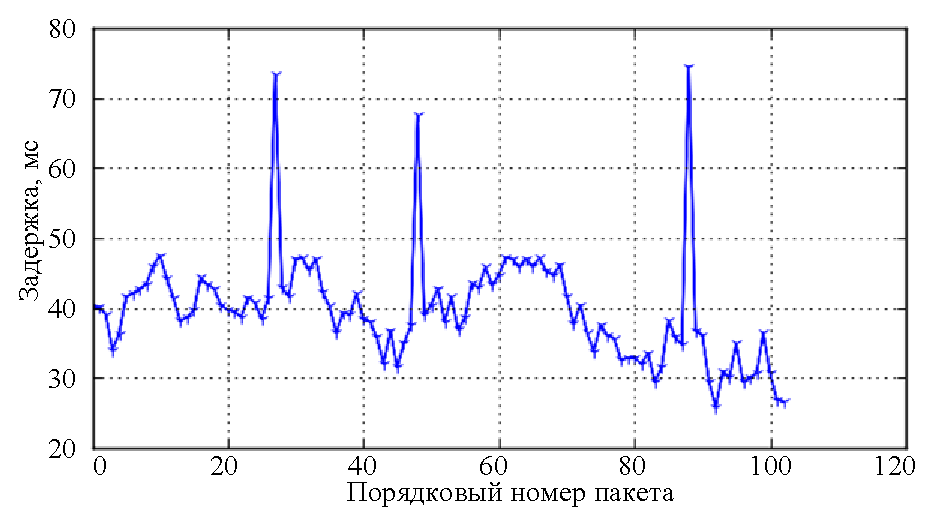
\includegraphics[width=1\linewidth , height=4.5cm]{3chapter/3_1_a.eps} а) \\
\end{minipage}
\hfill
\begin{minipage}[h]{0.47\linewidth}
\center
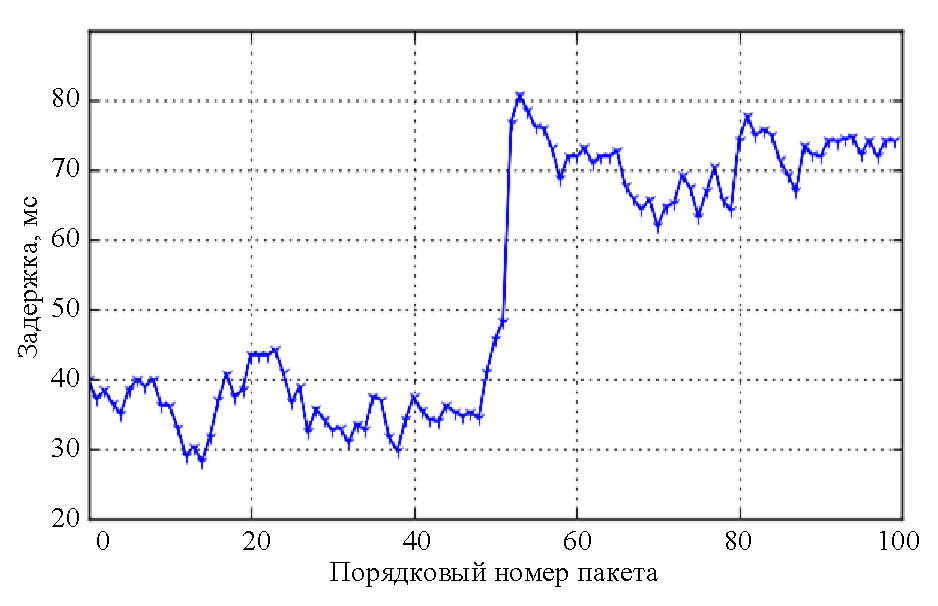
\includegraphics[width=1\linewidth, height=4.5cm]{3chapter/3_1_b.eps} б) \\
\end{minipage}
\caption{Моделирование ряда задержек a) с выбросами, б) со скачками}
\label{img3:modelJitter}
\end{figure}

В результате была получена математическая модель изменения задержки, которая будет использоваться в дальнейшем для моделирования буфера компенсации джиттера.





\section{Выводы ко второму разделу} \label{sect:concl2}

\begin{enumerate}
%\item Проведен анализ основных причин джиттера в проводной и беспроводной сети, который включает анализ таких причин, как перегрузки в канале доступа, внутрисистемные помехи, замирания в канале связи и т. д. Все это показывает, что такие современные сети, как LTE, остаются подвержены влиянию джиттера. На данный момент разработка алгоритмов, которые позволяют мониторить текущее состояние и решать проблему с джиттером и пакетными потерями для трафика реального времени является актуальной задачей.
\item 
Практика показывает, что наблюдаются три основные типа джиттра: постоянный джиттер, джиттер содержащий выбросы задержки и джиттер содержащий скачки задержки.
Подобная градация позволяет разработать дифференцированный подход к компенсации того или иного типа джиттера.
Соответственно требуется различный подход к компенсации джиттера при проявлении одного из этих трех типов джиттера.
Вместе с тем, сам рабочий алгоритм компенсации джиттера должен быть универсальным, обеспечивая автоматическое изменение функционирования при различных ситуациях.


\item Проведен анализ причин возникновения джиттера в гибридных сетях.
Эти причины различны и характерны для проводных и беспроводных сетей.
Также для каждой из этих причин определен характерный тип джиттера, согласно выбранной градации по трем основным типам.
Источником постоянного джиттера может являться пакетное планирование на стороне отправителя, балансировка нагрузки между несколькими линиями доступа или между различными маршрутами и внутреннее распределение нагрузки на маршрутизаторе.
Источником выбросов задержки могут являться перегрузки в локальной сети, влияние высокоприоритетного трафика на менее приоритетный и хэндовер между базовыми станциями.
Источником скачков задержки могут являться перегрузки в канале доступа, изменение расстояния между абонентом и базовой станцией, внутрисистемные помехи и замирания в радиоканале связи.
Наличие скачков и выбросов приводит к искажению, отклонению статистики от гауссовой, что в свою очередь приведет к потерям оптимальности алгоритма компенсации джиттера. 
Таким образом, возникает задача поиска методов решения для такой нестационарной ситуации и нахождение приемлемых подоптимальных решений.

\item На основании проведенного анализа синтезирована математическая динамическая модель процесса задержки, 
включающая постоянный джиттер, выбросы задержки и скачки задержки, на основе уравнения состояния и
уравнения наблюдения, отражающего процесс изменения состояния системы на фоне гауссовского белого шума.
Указанные выбросы следует включить в уравнение наблюдения так, как выброс задержки не должен влиять на состояние системы 
и будет учитывать при расчете буфера компенсации джиттера, как отклонение от текущего значения задержки.
При появлении скачка система компенсации джиттера должна учесть изменения джиттера и как можно раньше изменить размер буфера на необходимое значение, что обеспечит снижение задержки и пакетных потерь.
В связи, с чем скачки задержки введены в уравнение состояния.

\item Для борьбы с выбросами и скачками задержки имеет смысл применить следующую стратегию функционирования буфера компенсации джиттера.
Учитывая кратковременность действия единичного выброса и то, что система после его действия возвращается в первоначальное состояние, следует игнорировать выбросы при оценке текущего состояния системы,
а учитывать его в расчете буфера компенсации джиттера, как отклонение (дисперсию) от текущего состояния задержки.
В тоже время появление скачка имеет достаточную продолжительность и существенным образом изменяет наблюдаемую статистику, вследствие чего задачей синтезируемого метода будет являться изменение состояния системы на новое значение задержки.

\item Проведено моделирование процесса задержки на основе синтезированной математической модели, что показало адекватность полученной модели.
%\item На основе выше изложенного анализа, предлогаем разработать алгоритм компенсации джиттера и способ его эффективного внедрения в LTE сеть в разделе \ref{chapt3}.
\end{enumerate}

